\documentclass[letterpaper]{article}
\usepackage[left=1in,right=1in,top=1in,bottom=1in]{geometry}

\title{Outline for MOF energy histogram work}
\author{Ben Bucior, Scotty Bobbitt, Arun Gopalan, Neda Bagheri, Randy Snurr}

\usepackage[hidelinks]{hyperref}
\usepackage{graphicx}
\usepackage{amsmath}
\usepackage{comment}

\usepackage[section]{placeins}  % Float barrier between sections, per https://tex.stackexchange.com/questions/4854/floats-how-to-restrict-floating-to-subsection-only-in-one-section-of-the-docum

\usepackage{float} % Can force float locations for the outline.  Change back in the final template
% See also https://tex.stackexchange.com/questions/162284/non-floating-figures

\usepackage{outlines}
\usepackage{hyperref}
\usepackage{chemscheme}

\newcommand{\red}[1]{\textcolor{red}{#1}}

\begin{document}

\maketitle

%\begin{abstract}
%
%\end{abstract}

\section{Notes}
\begin{outline}
	\1 The Guest Editors Andrew Ferguson and Johannes Hachmann for the special issue chaired my session at AIChE.
	\1 Themed issue "Machine Learning and Data Science in Materials Design" for the journal \textit{Molecular Systems Design \& Engineering}
	\1 Filling in the outline with rough figures and ideas for the flow
\end{outline}


\section{Title}
\begin{outline}
	\1 (scratch work.  Let's come back to this later.)
	\1 (from AIChE) Identifying New Descriptors for Gas Storage in Nanoporous Materials
\end{outline}

\section{Requirements and future directions}

\subsection{Quick tasks for Ben}
\begin{outline}
	\1 Figure out in meeting: Do we pre-set the upper and/or lower bounds of the histograms?
	\1 Fitting models on the 2 bar and 100 bar cases.  Do the coefficients sum to the combined model?
		\2 Answer: yes.  I calculated a "discrepancy" term between the original ridge model and by subtracting the original high and low pressure models.  The max discrepancy between betas is 0.3 ("Inf" bin), which isn't unexpected considering we regularize the models separately.
		
		Also from the plot, we can observe properties of the individual fitted models.  Here, we can see that the highly attractive region actually has similar beta values.  The difference really comes into play at the mildly attractive regions, where adsorption is not sufficiently strong to bind H2 at 2 bar.  Also the "Inf" bin might be attributed to the differences in $\beta_0$, 41 vs. 17 g/L.
		\begin{figure}[H]
			%TODO: change this back in the manuscript document
			%\begin{figure}[!ht]
			\centering
			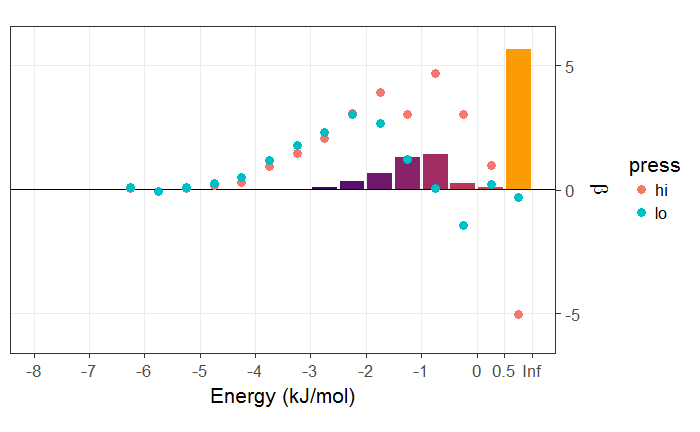
\includegraphics[width=0.75\columnwidth]{Figs/beta_vs_pressure.png}
			\caption{Difference between the beta coefficients at 2 bar and 100 bar (add this as a subfigure to the other beta plot?)}
			\label{fig:diff_betas}
		\end{figure}
	\1 Take a look at the \href{http://www.rsc.org/journals-books-databases/about-journals/molecular-systems-design-engineering/#undefined}{journal guidelines for authors} and their \href{http://www.rsc.org/journals-books-databases/journal-authors-reviewers/author-tools-services/#article-templates}{\LaTeX~templates}.  See also Overleaf?
\end{outline}

\subsection{Potential directions}
\begin{outline}
	\1 \textbf{How general} is the method?  Just hMOFs?  Also ToBaCCo?
		\2 Could retrain on ToBaCCo and compare coefs
		\2 IZA database of zeolites? (not just MOFs)
		\2 CCDC MOFs - test model on 1000 MOFs, check agreement, then screen the rest of them?
	\1 Identify old sources of \textbf{GCMC data for reuse} (email Diego or others?)
	\1 \textbf{Other gases:} methane
	\1 \textbf{Temperature dependence/optimization:} Cryo vs. room temperature adsorption?
		\2 Then, along with the story, we could see if the magnitude/direction of ridge regression coefficients match the intuition of needing stronger adsorption at higher temperature.
\end{outline}

\subsection{Other (unlikely) directions}
\begin{outline}
\1 \textbf{Experimental collaboration:} Screening the CCDC MOFs to identify top candidates for hydrogen storage (Would likely take a few weeks at best, so skip)
\1 \textbf{Isotherm prediction or Langmuir rationalization:} Repeat the predictions on multiple pressures.  What do the coefficients look like?  Comparison against isotherm prediction work?
\1 Other gases: xenon, multi-site molecules (large and complicated.  Let's save Xe/Kr for the isotherm prediction paper)
\end{outline}


\section{Introduction}

\begin{outline}
	\1 Hydrogen storage challenge
	\1 MOF background
	\1 Screening MOFs for hydrogen storage
		\2 Generating databases of hypothetical MOFs
		\2 Automating screening
		\2 More computationally efficient methods for screening
		\2 Scotty/Jiayi paper (agnostic binding fraction, JPCC)
		\2 Yamil, Diego works
	\1 Use of ML in the MOF literature
		\2 APRDF
		\2 Recent work from U Connecticut on textural properties + chemistry
		\2 Revisit my screening section in the \href{https://www.elsevier.com/books/modelling-and-simulation-in-the-science-of-micro-and-meso-porous-materials/catlow/978-0-12-805057-6}{review book} for more ideas on papers to cite
		\2 Use of potentially related features in the literature, like the Coulomb matrix, heat of adsorption, etc.
	\1 Current paper not only shows potential for accelerating MOF screening but also learning what is driving the capacity of these materials
		\2 Accelerate beyond brute force GCMC
		\2 LJ metric and ridge regression get to the heart of what makes a good material (avoids problem of void fraction peak).  Higher metric = higher capacity
\end{outline}



\section{Methods}

TODO:
Flip sections 5.1 and 5.2.  Rewrite them as:
\begin{enumerate}
	\item Data collection (GCMC, DB, grid, z-scoring, etc.)
	\item Data analysis (ridge, etc.--error handling?)
	\item Data sharing (consider making the GCMC and PES data publicly available.  Also could make a quick web interface where users can make predictions on their own MOF)
\end{enumerate}

\subsection{Calculating the energy grid}

\begin{figure}[H]
%TODO: change this back in the manuscript document
%\begin{figure}[!ht]
	\centering
	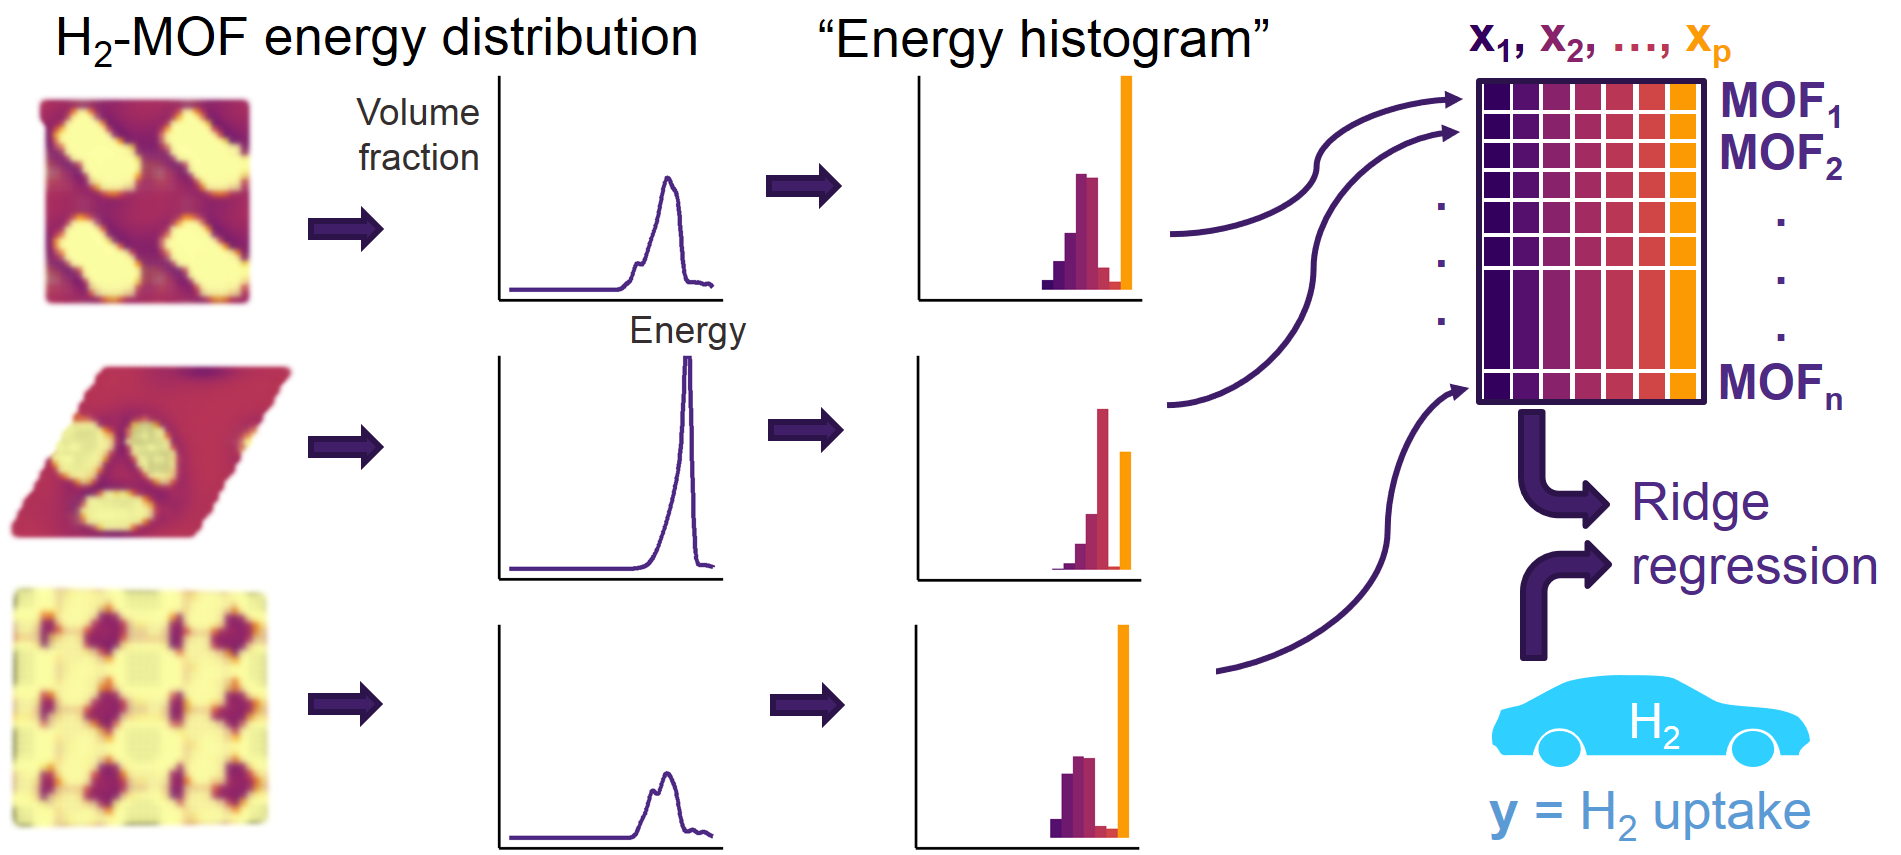
\includegraphics[width=0.75\columnwidth]{Figs/energy_schematic.png}
	\caption{Calculation of the energy histogram from inputs}
	\label{fig:schematic}
\end{figure}


\subsection{Molecular simulations}

\begin{outline}
	\1 RASPA
	\1 Force field parameters for host and guests
	\1 Number of cycles and/or source of data
	\1 Structures
		\2 Wilmer's hMOFs
		\2 Likely ToBaCCo, so we can also look at structural diversity
		\2 Cleaning up the CCDC MOF subset using their solvent removal scripts, etc.
\end{outline}


\subsection{Data processing}

\begin{outline}
	\1 Ridge regression
		\2 Equations and loss function
		\2 R package \verb|glmnet|
			\3 Finding the greatest lambda within 1 SE of the lambda that minimizes model error
			\3 [Can probably keep this vague-ish, since we'll be citing a known package]
	\1 Data preprocessing: z-score bins and remove columns with zero variance.  Also filter out unphysical uptake ($<$ 0 g/L) from GCMC
	\1 Define equations used for model evaluation: Q2, RMSE, MAE [move to results, as necessary]
\end{outline}



\section{Results and discussion}

\subsection{LJ metric [we'll see where this fits best in the flow]}

\begin{outline}
	\1 Inspiration from "binding fraction"
		\2 A similar idea, but calculated using interaction energy instead of geometry
		\2 Set two cutoffs on the energy distribution, and integrate between them to get a single value.
	\1 Describe graphene sheet calculation, showing the 7 Ang and the other cutoff, and how they correspond with our energies empirically derived
\end{outline}

\begin{figure}[H]
	\centering
	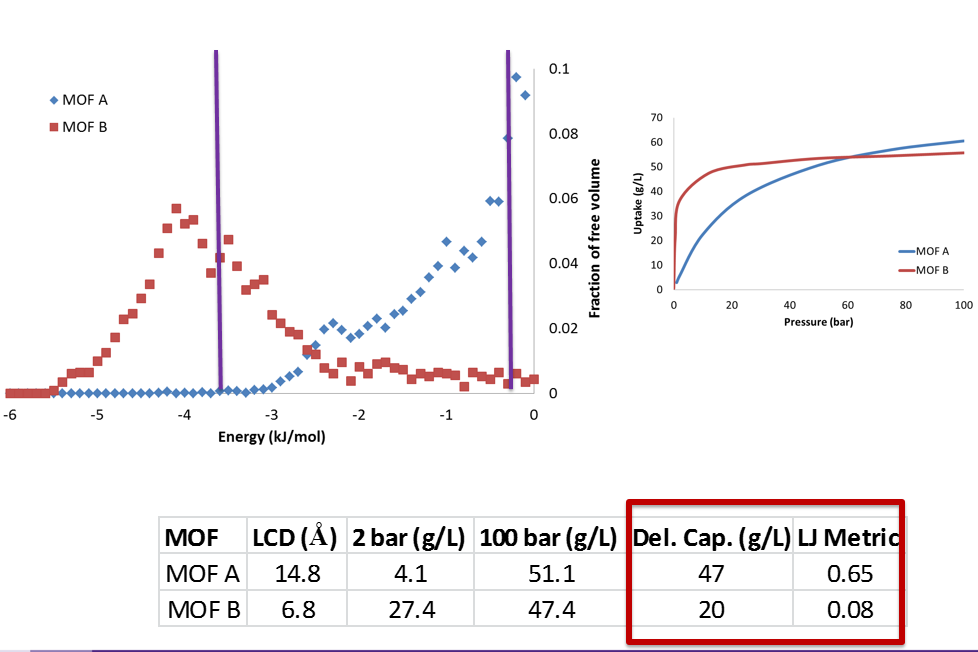
\includegraphics[width=0.75\columnwidth]{Figs/binding_case_study.png}
	\caption{Case study of two MOFs (IDs?) demonstrating that deliverable capacity also depends on the absolute uptake of the delivery pressure.  Note that MOFs A and B have similar saturation loadings, but considerably different deliverable capacity due to uptake at the low delivery pressure (REDO)}
	\label{fig:binding_cases}
\end{figure}

\begin{figure}[H]
	\centering
	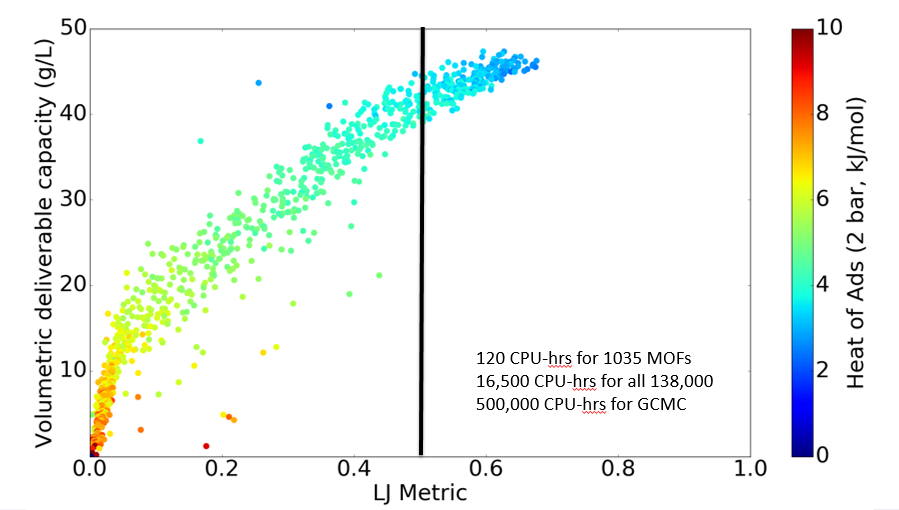
\includegraphics[width=0.75\columnwidth]{Figs/lj_metric.png}
	\caption{The LJ metric generally indicates deliverable capacity.  Each point represents results for one of $\approx 1000$ hMOFs tested. [ADD DC VS. VF PLOT as another subfigure]}
	\label{fig:lj_metric}
\end{figure}

\subsection{Ridge regression}
\begin{outline}
	\1 Formalizing the results from LJ metric studies in a predictive model without empirical parameter determination
	\1 Meaning of betas and intuition
	\begin{figure}[H]
		\centering
		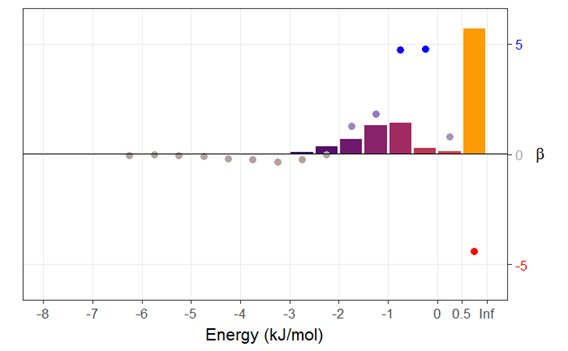
\includegraphics[width=0.75\columnwidth]{Figs/betas.png}
		\caption{Regression coefficients overlaid on the histogram}
		\label{fig:betas}
	\end{figure}
	\1 How good is the model and fit?
		\2 Parity plot
		\begin{figure}[H]
			\centering
			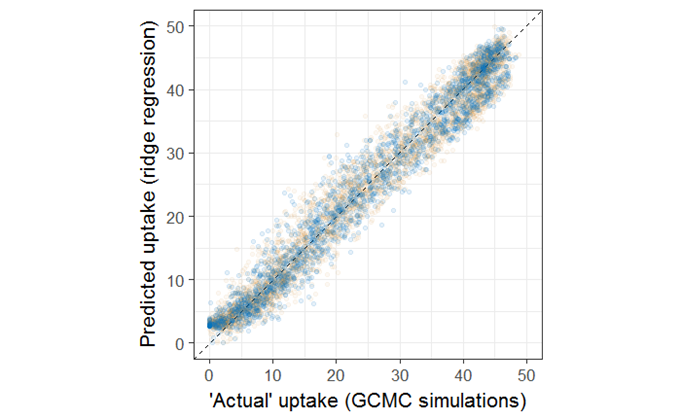
\includegraphics[width=0.75\columnwidth]{Figs/parity.png}
			\caption{Parity plot for (a) training and (b) test data on the energy histograms (TODO: split into two subfigures so it's easier to read without an animation.)}
			\label{fig:parity}
		\end{figure}
		\2 Q2 of 0.96
		\2 RMSE of 3 g/L, MAE/MUE of 2.4 g/L
	\1 Why ridge regression?
		\2 Interpretability with a simple model
		\2 Likely some kind of link with a multi-site Langmuir model (assuming that all sites at a given energy are identical)
		\2 Someone at AIChE asked why our model didn't include nonlinearity.  The reason is that we don't need that to make great predictions. (some of my initial work used random forest, which would avoid manual feature transformations)
\end{outline}

\begin{figure}[H]
	\centering
	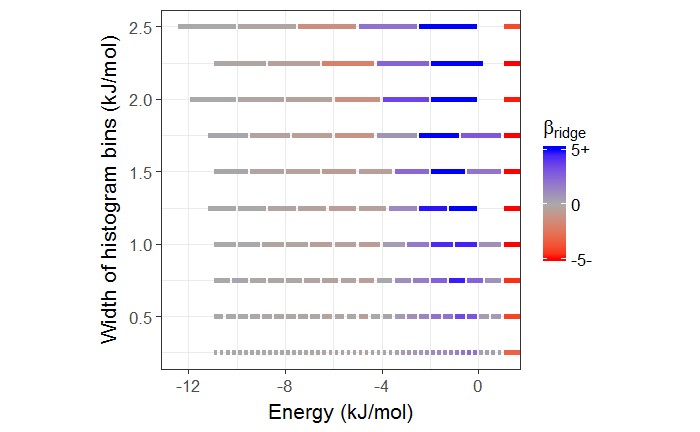
\includegraphics[width=0.75\columnwidth]{Figs/beta_robustness.png}
	\caption{DEMO Model coefficients are robust to histogram bin strategy: showing the locations of the bins, color coded by the beta, to see if the model gives consistent results for certain sections of energy (TODO after meeting)}
	\label{fig:binwidth}
\end{figure}

\subsection{Screening other databases}
\begin{outline}
	\1 Plan of testing applicability on 1000 MOFs
	\1 Benchmarking (maybe as a table): Full GCMC vs. energy grid calculations, feature representation, and ML
	\1 TODO: pick out the top 500 CSD MOFs and test them with GCMC
\end{outline}
\begin{figure}[H]
	\centering
	\caption{TODO: top candidates for experimental synthesis based on screening the CCDC MOF database (MAYBE?)}
	\label{fig:candidates}
\end{figure}

\subsection{Generalizability to other gases}
\begin{outline}
	\1 Methane. See above
\end{outline}

\subsection{Other figures}
The last two sections will naturally lend themselves to additional figures as well.

\section{Acknowledgements}
Data Science Initiative, NMGC, etc.


\pagebreak
\section{Supporting Info}

\subsection{Hyperparameter tuning}

\begin{outline}
	\1 Grid spacing: convergence of a few different sample MOF histograms
		\2 Also might be good to have a figure overlaying sampling points on top of a continuous background, to exemplify the convergence testing
		\2 TODO make a figure more rigorously
	\1 Bin width and degree of overlap (TODO: consider adding examples, and Q2 figure)
	\1 Lambda selection
	\begin{figure}[H]
		\centering
		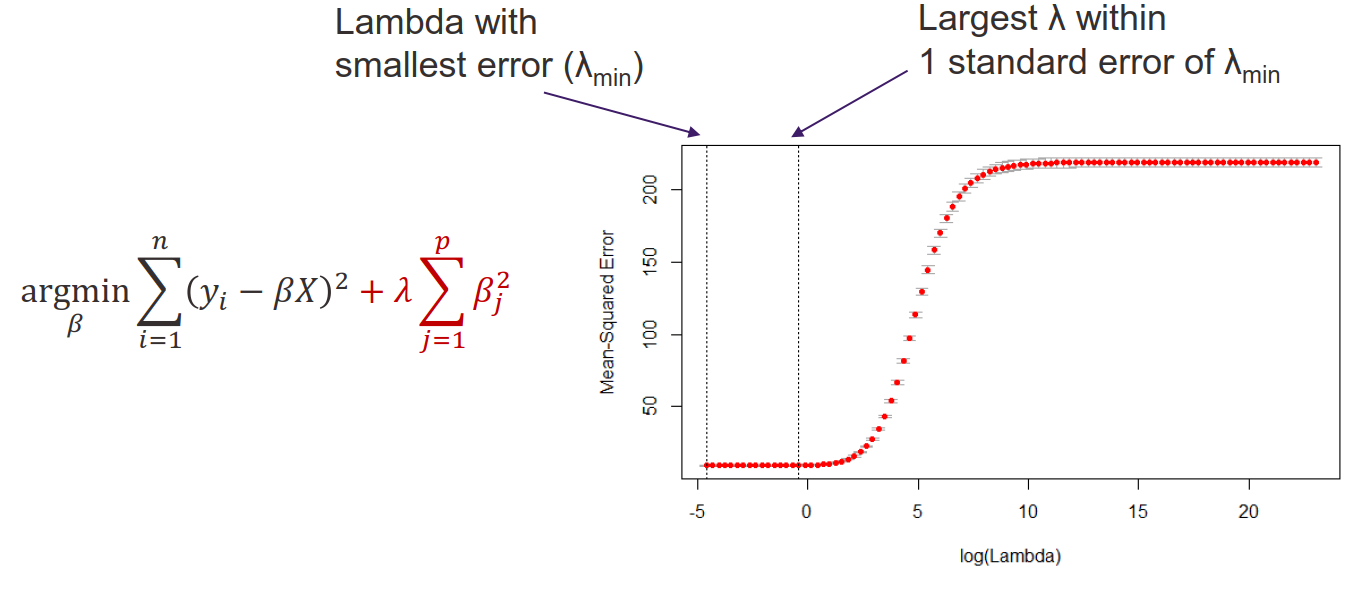
\includegraphics[width=0.75\columnwidth]{Figs/lambda.png}
		\caption{Determination of the regularization parameter $\lambda$ for ridge regression}
		\label{fig:lambda}
	\end{figure}
\end{outline}

\begin{figure}[H]
	\centering
	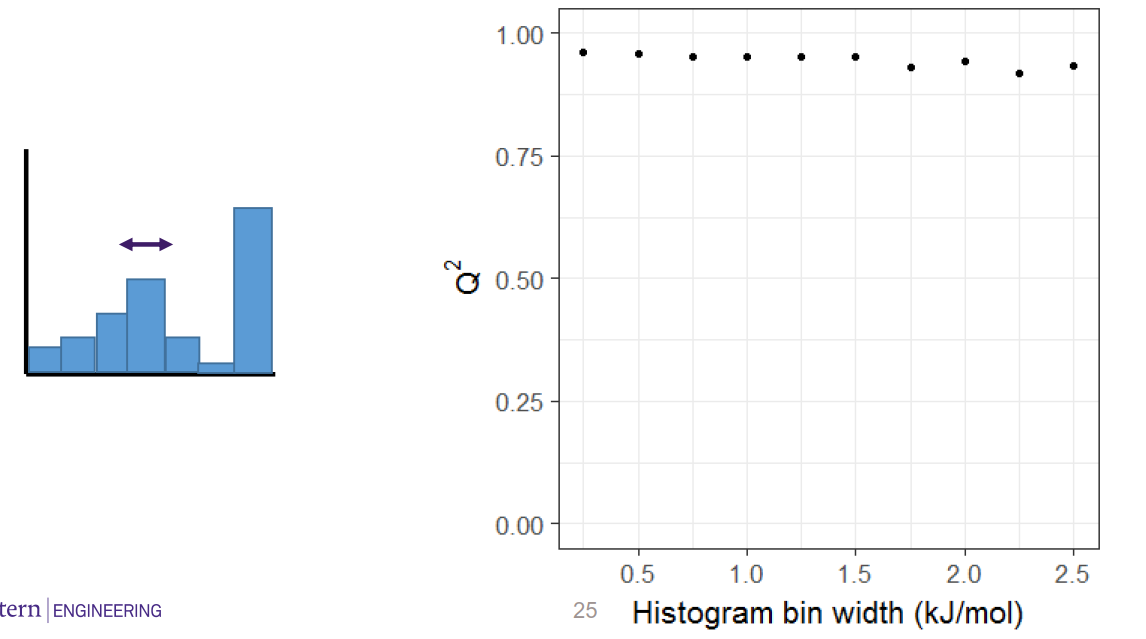
\includegraphics[width=0.75\columnwidth]{Figs/tuning_bin_width.png}
	\caption{Model is robust to selected histogram bin width (perhaps repeat with RMSE in addition to Q2)}
	\label{fig:robustness_q2}
\end{figure}

\subsection{Model evaluation/consistency}

Also consider adding a figure on "Consistency across nodes/linkers and/or other DBs" (see Zr results)

\begin{figure}[H]
	\centering
	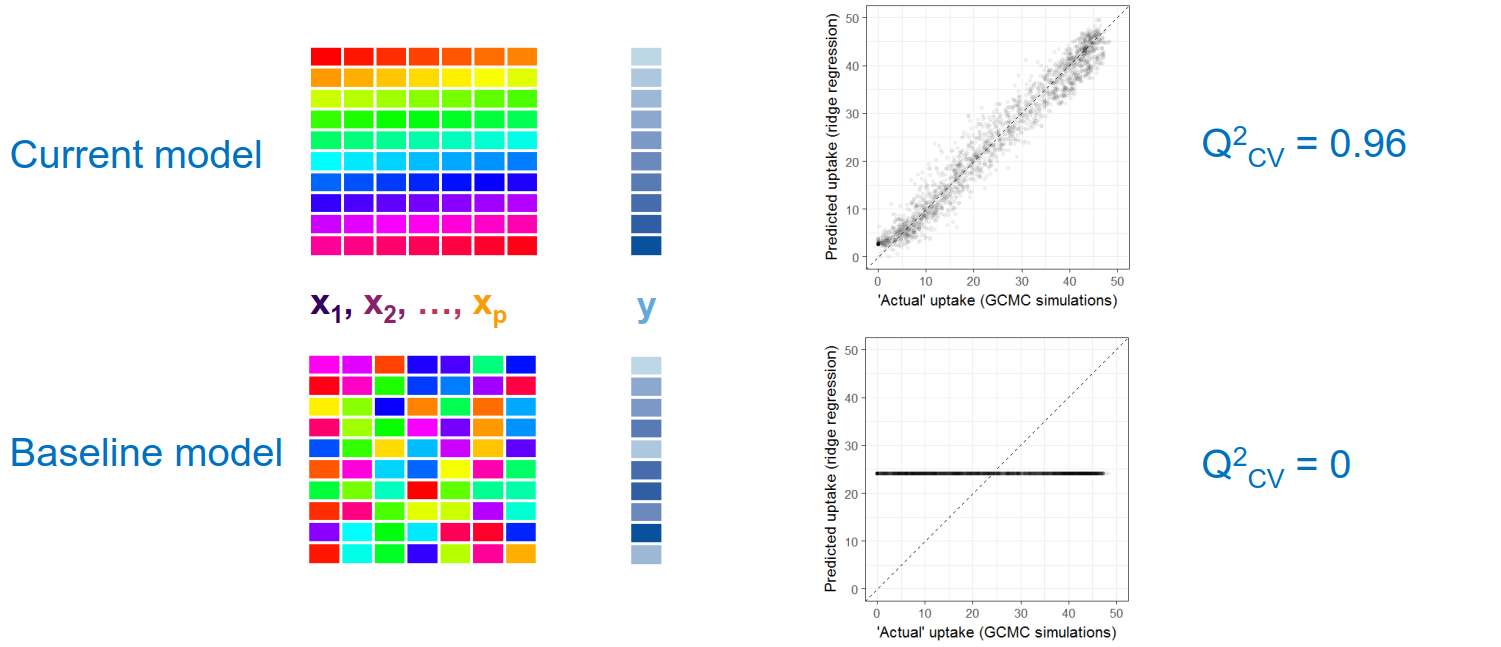
\includegraphics[width=0.75\columnwidth]{Figs/random_baseline.png}
	\caption{Comparison of $Q^2$ against a baseline of random data}
	\label{fig:q2_baseline}
\end{figure}

\begin{figure}[H]
	\centering
	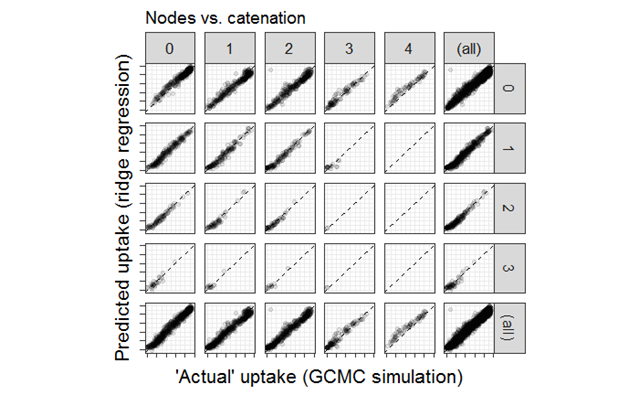
\includegraphics[width=0.75\columnwidth]{Figs/consistency_across_compositions_p.png}
	\caption{Consistency of model accuracy across MOF compositions.  Note that Zr MOFs are less accurate (node 4), possibly due to differences in topology and undersampling relative to \textbf{pcu} MOFs.}
	\label{fig:nodes_vs_cat}
\end{figure}

\begin{figure}[H]
	\centering
	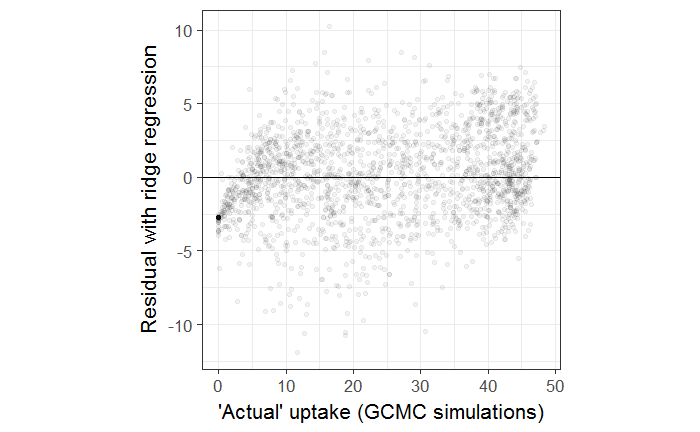
\includegraphics[width=0.75\columnwidth]{Figs/residual.png}
	\caption{Residual plot for the testing data.  One audience member in my talk once concerned about a long tail (?) on the top right of my parity plot, below the line of parity, possibly requiring another variable for correction.  But I'm having trouble seeing it in the residual plot, so perhaps it was an optical illusion against the 45 degree line.}
	\label{fig:test_residual}

[TODO: also fit the residuals to a Gaussian to verify that there isn't a problem with top right]

\end{figure}


\subsection{Alternative approaches}

\begin{outline}
	\1 Benchmarking against traditional descriptors (textual properties like void fraction and density)
	\begin{figure}[H]
		\centering
		%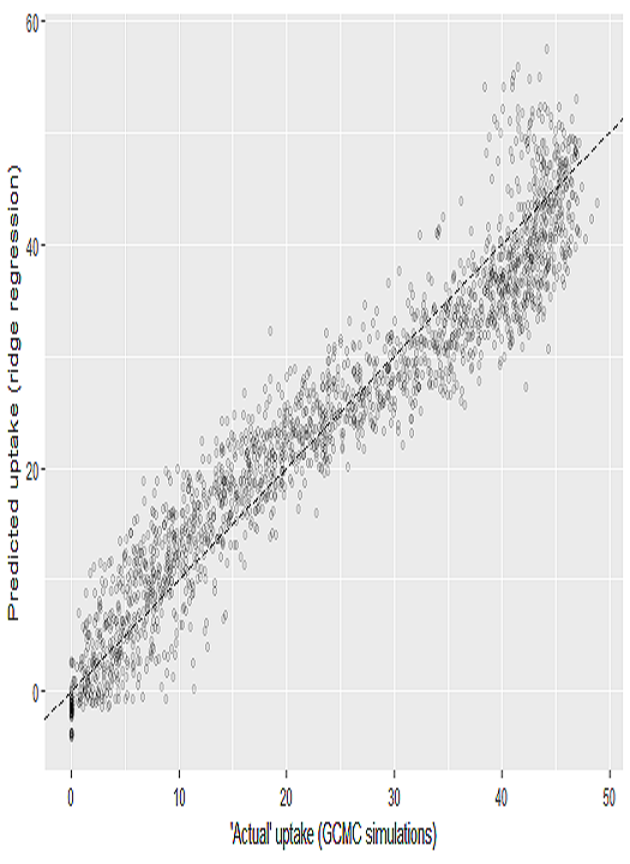
\includegraphics[width=0.75\columnwidth]{Figs/textural_prediction.png}
		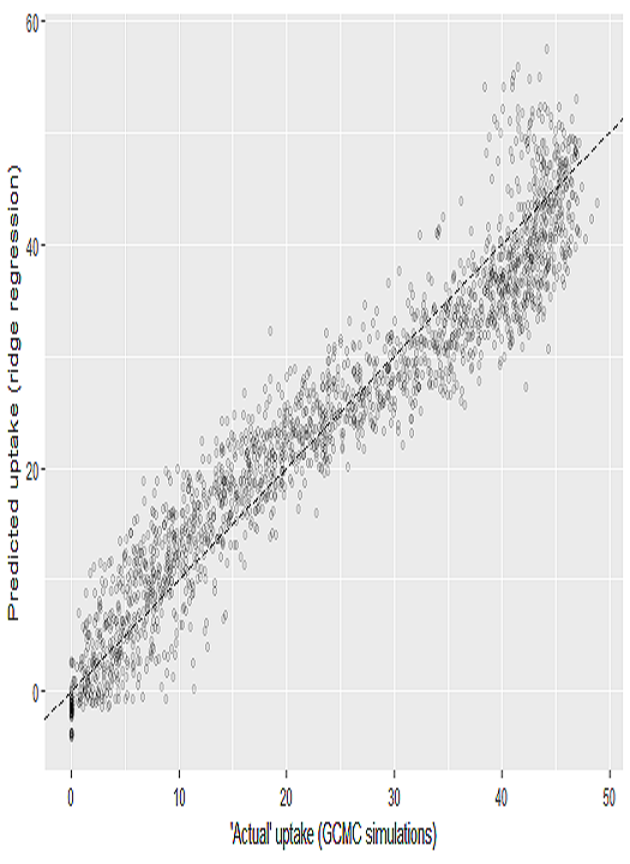
\includegraphics[width=0.5\columnwidth]{Figs/textural_prediction.png}
		\caption{Textural properties (void frac, grav SA, vol SA, DPD, LCD, max catenation, and actual catenation) have poorer predictivity.  On the test set, RMSE=4.3, MAE=3.5, and note the uneven residuals. (from 10/06, need to replot)}
		\label{fig:textural}
	\end{figure}
	\1 LASSO figure and coefficients
	\begin{figure}[H]
		\centering
		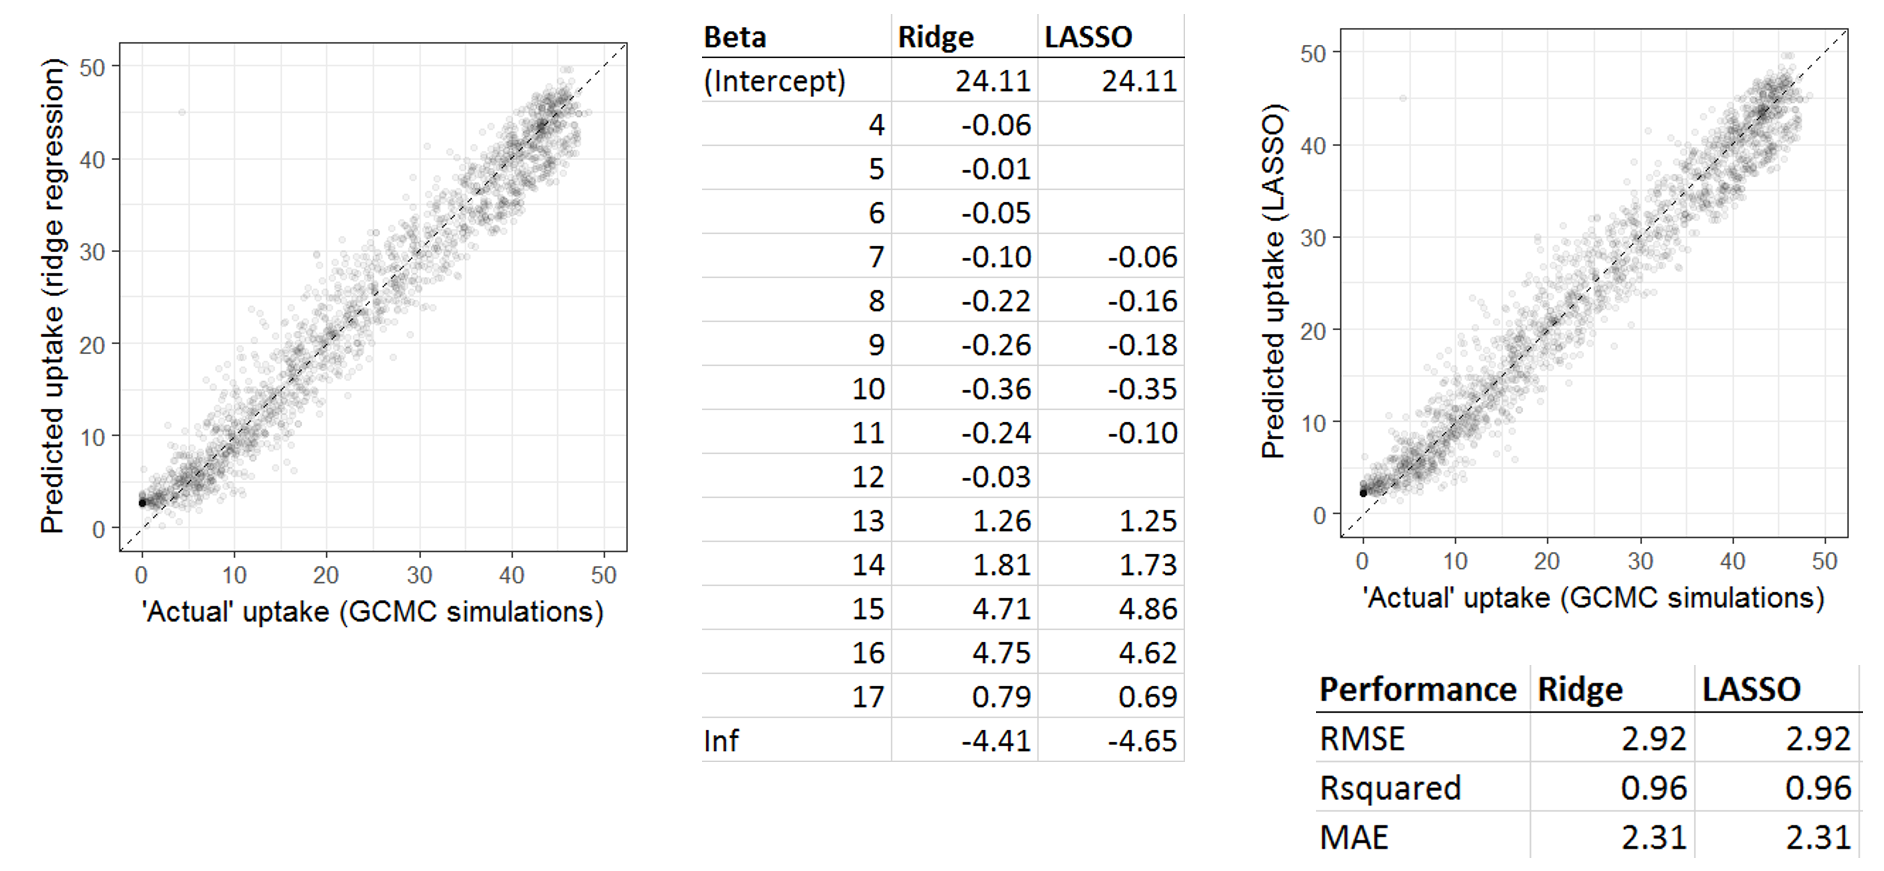
\includegraphics[width=0.75\columnwidth]{Figs/ridge_vs_lasso.png}
		\caption{Ridge regression and LASSO give similar results}
		\label{fig:lasso}
	\end{figure}
	
\end{outline}


\subsection{Some newer figures on normality and transferability}
How well does the model work on a set of new 500 CCDC MOFs?  The left subfigure speaks for itself.

The discrepancy could be a number of causes: first we need to check the sigma/epsilon parameters for the energy calculations.  The original 10k hMOFs used an epsilon of 11.25~K and sigma of 2.68~Angstroms, but the actual sigma was about 36.7~K.  After correction, the fit is considerably better (right subfigure).  For the remainder of the error, consider that we mostly trained on **pcu** MOFs, whereas the CCDC MOFs are considerably more diverse.

\begin{figure}[H]
	\centering
	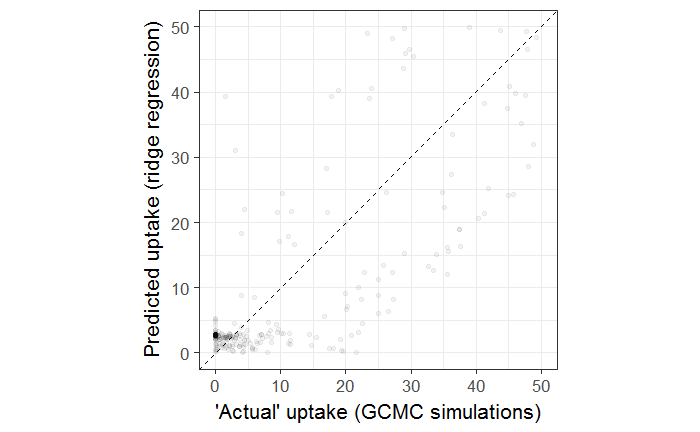
\includegraphics[width=0.75\columnwidth]{Figs/initial_ccdc.png}
	\caption{Parity plot for the CCDC MOFs, using the initial ridge regression model trained on 4000 hMOFs.}
	\label{fig:init_ccdc_parity}
\end{figure}

\begin{figure}[H]
	\centering
	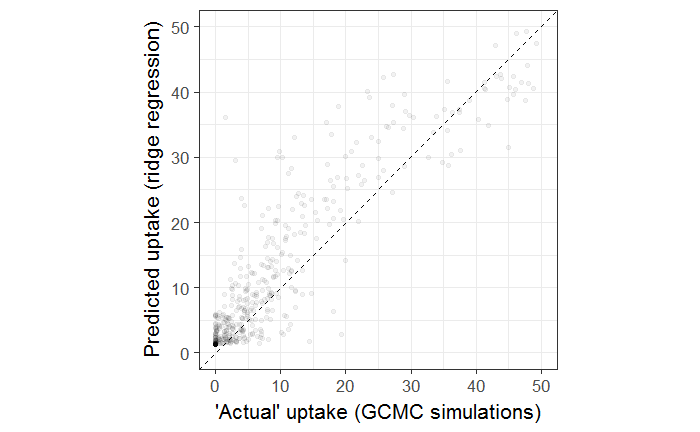
\includegraphics[width=0.75\columnwidth]{Figs/initial_ccdc_scaled_hmof.png}
	\caption{Parity plot for the CCDC MOFs, after scaling the energies fed to the hMOF ridge regression model to match epsilon.}
	\label{fig:init_ccdc_parity}
\end{figure}

Let's take a look at the distribution of z-scores.  Do high or low performing MOFs tend to have similar z-scores in certain bins?  Are the z-scores reasonable (especially for "important" bins)?
\begin{figure}[H]
	\centering
	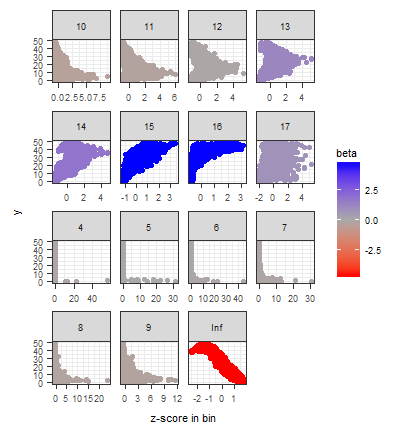
\includegraphics[width=0.47\columnwidth]{Figs/z_distr.png}
	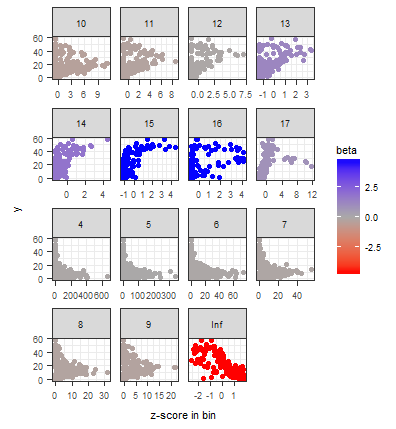
\includegraphics[width=0.47\columnwidth]{Figs/z_distr_init_ccdc.png}
	\caption{Distribution of z-scores (x variables) in each bin, colored by the beta of the trained model.  Extreme z-scores are more common in the bins with low weights.  Left: original hMOF data, right: CCDC vs. actual GCMC, with the new betas (from scaled hMOF energies)}
	\label{fig:z_distr}
\end{figure}






\end{document}
